\documentclass[tikz, border=8pt]{standalone}
\usepackage{amsmath}

\begin{document}
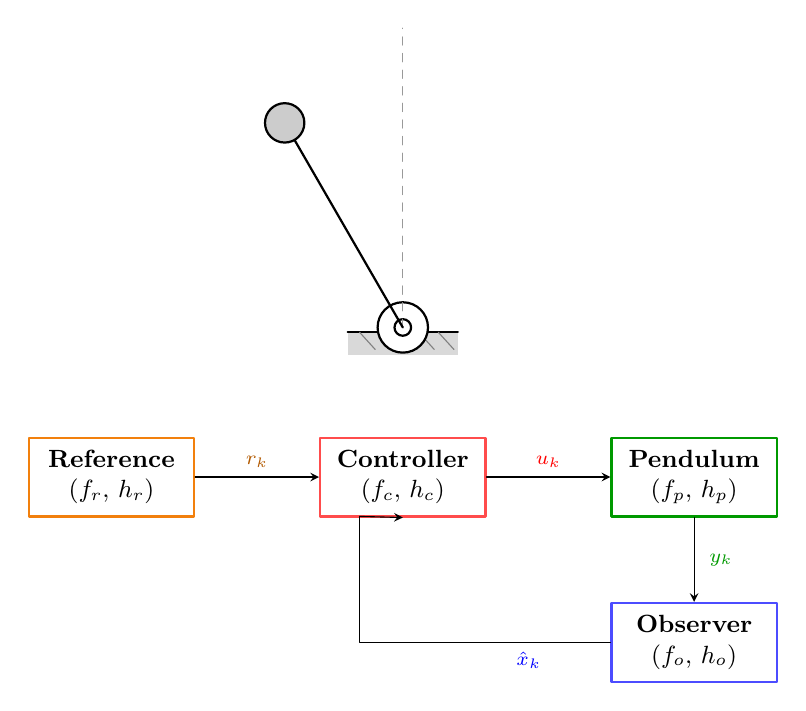
\begin{tikzpicture}[
  line cap=round, line join=round, >=stealth,
  blk/.style={draw, thick, minimum width=2.1cm, minimum height=1.0cm,
              align=center, fill=white, font=\small}
]

  % ── Inverted pendulum ─────────────────────────────────────────────────────

  % Floor mount
  \fill[black!15] (-0.7, -0.35) rectangle (0.7, -0.06);
  \draw[thick] (-0.7, -0.06) -- (0.7, -0.06);
  \foreach \xi in {-0.55,-0.30,-0.05,0.20,0.45}
    \draw[thin, black!50] (\xi, -0.06) -- ++(0.20, -0.22);

  % Motor
  \filldraw[fill=white, draw=black, thick] (0,0) circle (0.32);
  \filldraw[fill=white, draw=black, thick] (0,0) circle (3pt);

  % Dashed vertical
  \draw[dashed, black!40, thin] (0,0) -- (0,3.8);

  % Rod
  \draw[thick] (0,0) -- (-1.5, 2.598);

  % Bob
  \filldraw[fill=black!20, draw=black, thick] (-1.5, 2.598) circle (0.25);

  % ── Feedback block diagram ─────────────────────────────────────────────────
  %
  %   [Reference] --r_k--> [Controller] --u_k--> [Pendulum]
  %                              ^                    |
  %                              |                   y_k
  %                              |                    |
  %                         x_hat_k               [Observer]
  %                              |                    |
  %                              +--------------------+

  \node[blk, draw=orange!80!brown] (ref)   at (-3.7, -1.9)
      {\bfseries Reference\\\normalfont$(f_r,\,h_r)$};
  \node[blk, draw=red!70]          (ctrl)  at (0,    -1.9)
      {\bfseries Controller\\\normalfont$(f_c,\,h_c)$};
  \node[blk, draw=green!60!black]  (plant) at (3.7,  -1.9)
      {\bfseries Pendulum\\\normalfont$(f_p,\,h_p)$};
  \node[blk, draw=blue!70]         (obs)   at (3.7,  -4.0)
      {\bfseries Observer\\\normalfont$(f_o,\,h_o)$};

  % r_k: Reference → Controller
  \draw[->] (ref.east) -- (ctrl.west)
    node[midway, above, font=\scriptsize\itshape, orange!70!black] {$r_k$};

  % u_k: Controller → Plant
  \draw[->] (ctrl.east) -- (plant.west)
    node[midway, above, font=\scriptsize\itshape, red] {$u_k$};

  % y_k: Plant → Observer (straight down)
  \draw[->] (plant.south) -- (obs.north)
    node[midway, right=2pt, font=\scriptsize\itshape, green!60!black] {$y_k$};

  % x̂_k: Observer.west → left → up → ctrl.south
  \draw (obs.west) -- (-0.55, -4.0) -- (-0.55, -2.4);
  \draw[->] (-0.55, -2.4) -- (ctrl.south);
  \node[below, font=\scriptsize\itshape, blue] at (1.6, -4.0) {$\hat{x}_k$};

\end{tikzpicture}
\end{document}
